\chapter{GIAO TIẾP RS232}
\label{chapter:rs232}
\section{Giới thiệu chung}
\subsection{Yêu cầu}
Giao tiếp giữu máy tính và vi điều khiển PIC 16F887 thông qua module RS232.
\subsection{Module RS232}
Cổng nối tiếp RS232 được sử dụng để kết nối các thiết bị ngoại vi với máy tính.

Ưu điểm: Khả năng chống nhiễu cao, tháo rời ra khỏi máy tính dễ dàng, cổng nối tiếp còn là nguồn cấp cho vi điều khiển,\ldots

Cách kết nối: Ta sử dụng 2 chân \verb|RX| và \verb|TX| của module kết nối lần lượt với 2 chân \verb|RX| và \verb|TX| của vi điều khiển (kết nối nối tiếp \verb|RX - RX| và \verb|TX - TX|).
\section{Các lệnh giao tiếp RS232}
Ta sử dụng khai báo và các lệnh sau để giao tiếp với RS232 qua cổng nối tiếp:
\begin{itemize}
\item Khai báo:
\begin{itemize}
\item Khai báo tần số thạch anh: \verb|#use delay(clock = 20000000)|, ví dụ tần số là $20MHz$
\item Khai báo RS232: 

\verb|#use RS232(BAUD = 9600, PARITY = N, XMIT = PIN_C6, RCV = PIN_C7)|

với \verb|BAUD = 9600|: tốc độ truyền; \verb|PARITY = N|: không kiểm tra chẳn lẻ; \verb|XMIT = PIN_C6|: chân truyền là \verb|C6|; \verb|RCV = PIN_C7|: chân nhận là \verb|C7|.
\end{itemize}
\item Các lệnh giao tiếp: \verb|printf|, \verb|getc|, \verb|getch|, \verb|getchar|, \verb|fgetc|, \verb|gets|, \verb|fgets|, \verb|puc|, \verb|putchar|, \verb|fputc|, \verb|puts|, \verb|fputs|, \verb|kbhit|, \verb|assert|, \verb|perror|, \verb|set_uart_speed|, \verb|setup_uart|.
\end{itemize}
\section{Bài tập}
\subsection{Bài tập 7.1}
\paragraph{Yêu cầu}Viết chương trình truyền dữ liệu giữa PC và PIC 16F887 với yêu cầu sau:
Truyền ký tự \verb|'b'| và \verb|'t'| từ PC thông qua chương trình MATLAB, khi PIC nhận được ký tự \verb|'b'| thì bật các LED ở PORT E, khi nhận được ký tự \verb|'t'| thì tắt các LED ở PORT E.
\paragraph{Hướng giải quyết}
\begin{itemize}
\item Chúng ta thực hiện truyền dữ liệu qua cổng nối tiếp RS232 để thực hiện giao tiếp giữa PC và PIC.
\item Khai báo RS232: chọn tốc độ truyền là \verb|9600|

\verb|#use RS232(BAUD = 9600, PARITY = N, XMIT = PIN_C6, RCV = PIN_C7)|
\item Sử dụng ngắt nhận dữ liệu từ RS232 là \verb|#INT_RDA|.
\begin{itemize}
\item Khai báo ngắt: 

\verb|ENABLE_INTERRUPTS(INT_RDA);| và \verb|ENABLE_INTERRUPTS(GLOBAL);|
\item Chương trình ngắt: 
\begin{itemize}
\item Nội dung chương trình ngắt:
\begin{itemize}
\item[+] Đọc giá trị từ PC gửi qua PIC: \verb|value = getc();|
\item[+] Nếu \verb|value = 'b'| thì đưa PORT E lên mức cao: \verb|PORTE = 0xFF;|
\item[+] Nếu \verb|value = 't'| thì đưa PORT E lên mức thấp: \verb|PORTE  0x00;|
\end{itemize}
\end{itemize}
\end{itemize}
\item Khai báo PORT E là OUTPUT: \verb|TRISE = 0x00;|
\item Sử dụng phần mềm MATLAB để gửi dữ liệu đến PIC:
\begin{itemize}
\item Xác định  tên cổng nối tiếp , ta dùng \verb|s = serial(tên_port,tốc_độ_truyền)| với Windows thì \verb|tên_port = 'com1'| (còn những hệ điều hành khác, chúng ta có thể xem hướng dẫn về \verb|serial| trong phần \verb|Help| của MATLAB); \verb|tốc_độ_truyền| bằng tốc độ truyền ta khai báo trong chương trình CCS. 
\item Mở port dùng: \verb|fopen(s)|.
\item Gửi giá trị qua port dùng: \verb|fprintf(s,'giá_trị_gửi')|.

Ví dụ: \verb|fprintf(s,'b')|.
\item Nếu không gửi dữ liệu tiếp, ta thực hiện đóng port dùng: \verb|fclose(s)|.
\end{itemize}
\end{itemize}
\newpage
\subsection*{Sơ đồ mạch}
\begin{figure}[!h]
\begin{center}
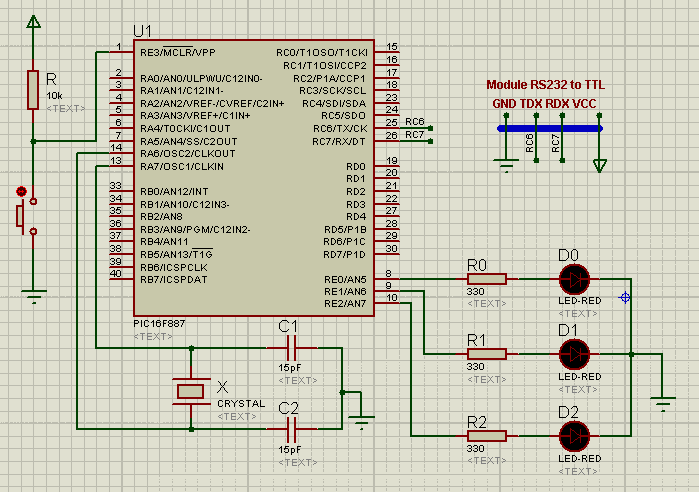
\includegraphics[scale=0.6]{bai-7/image/BAI-7-1}
\end{center}
\caption{Mạch sử dụng module RS232 to TTL nhận lệnh từ PC bật tắt LED ở PORT E}
\end{figure}
\subsection*{Chương trình 20}
\lstinputlisting[language=C]{BAI-7-1.C}

Chương trình nhận lệnh điều khiển từ PC với code Matlab (thực hiện lần lượt các lệnh sau bằng \verb|Command line|):
\lstinputlisting[language=Matlab]{BAI-7-1.m}
\subsection{Bài tập 7.2}
\paragraph{Yêu cầu}Viết chương trình truyền chuỗi \verb|"TT VI DIEU KHIEN"| từ PC xuống máy tính và hiển thị chuỗi nhận được lên LCD 16x02.
\paragraph{Hướng giải quyết}
\begin{itemize}
\item[$\ast$] Chúng ta dựa vào \textit{chương trình 20}, nhưng thay đổi một số chỗ cho phù hợp.
\item \textit{Chương trình ngắt}: Để đọc được một chuỗi từ PC truyền xuống, dùng hàm \verb|gets(string)| thay cho hàm \verb|getc()| (chỉ đọc được 1 ký tự).
\item \textit{Chương trình chính}: ta thêm các lệnh khởi tạo LCD (thêm vào thư viện \verb|LCD_LIB4BIT.C| ở phần khai báo đầu). Trong vòng lặp \verb|while| cho hiển thị chuỗi \verb|"TT VI DIEU KHIEN"| nhận được từ PC lên LCD.
\item[$\ast$] Khi chạy thực tế, đôi khi phần cứng bị nhiễu, đã nhận được chuỗi ký tự nhưng mà chưa hiển thị lên LCD thì nhấn nút Reset là chuỗi được hiển thị lên LCD.
\end{itemize}
\newpage
\subsection*{Sơ đồ mạch}
\begin{figure}[!h]
\begin{center}
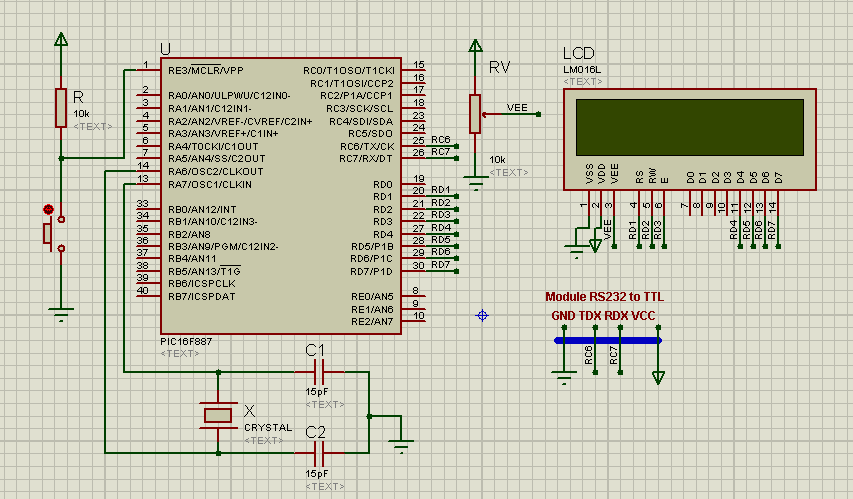
\includegraphics[scale=0.6]{bai-7/image/BAI-7-2}
\end{center}
\caption{Mạch sử dụng module RS232 to TTL nhận chuỗi từ PC hiển thị lên LCD}
\end{figure}
\subsection*{Chương trình 21}
\lstinputlisting[language=C]{BAI-7-2.C}

Chương trình nhận lệnh điều khiển từ PC với code Matlab (thực hiện lần lượt các lệnh sau bằng \verb|Command line|):
\lstinputlisting[language=Matlab]{BAI-7-2.m}
\subsection{Bài tập 7.3}
\paragraph{Yêu cầu}Viết chương trình đọc giá trị nhiệt độ từ IC TC74 sau đó truyền giá trị đọc được lên PC qua cổng RS232.
\paragraph{Hướng giải quyết}
\begin{itemize}
\item Do không có IC TC74, nên em thay thế bằng phần cứng khác là IC DS3231 (trong \textit{bài tập 6.2} và \textit{bài tập 6.3} \textit{trang \pageref{Ex:ds3231-1}} và \textit{trang \pageref{Ex:ds3231-2}}), nó có chức năng lưu thời gian thực và đọc nhiệt độ môi trường. 
\item Sự dụng IC với chức năng đọc nhiệt độ (trong \textit{bài tập 6.3 trang \pageref{Ex:ds3231-2}}) nên chúng ta rút ngắn lại \textit{chương trình 19 trang \pageref{code-19}}.
\item Sau khi đọc được nhiệt độ dùng lệnh \verb|printf("%.1fC", getTemp());| để gửi lên máy tính.
\item Sử dụng LCD để kiểm chứng lại kết quả gửi lên máy tính.
\item Phần code Matlab hoàn toàn giống \textit{bài tập 4.3 trang \pageref{Ex:4-3}}.
\end{itemize}
\newpage
\subsection*{Sơ đồ mạch}
\begin{figure}[!h]
\begin{center}
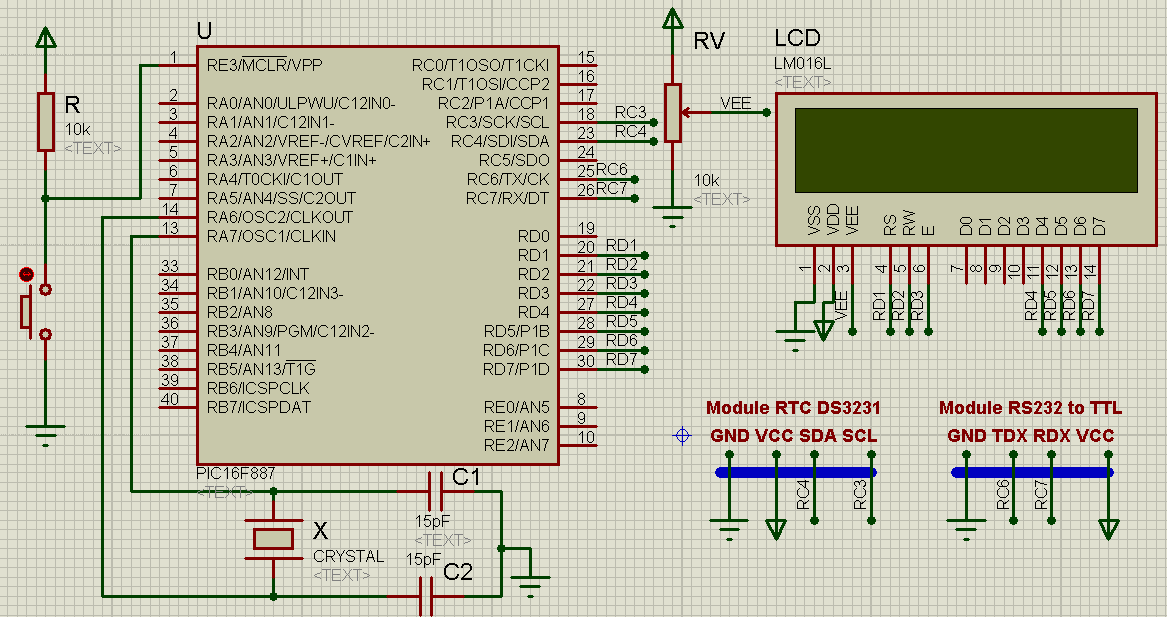
\includegraphics[scale=0.5]{bai-7/image/BAI-7-3}
\end{center}
\caption{Mạch sử dụng module RS232 to TTL gửi nhiệt độ từ IC DS3231 lên PC}
\end{figure}
\subsection*{Chương trình 22}
\lstinputlisting[language=C]{BAI-7-3.C}

Hàm \verb|Serial_Callback| dùng để thiết lập cho tham số \verb|BytesAvailableFcn| trước khi mở cổng COM:
\lstinputlisting[language=Matlab]{Serial_Callback.m}

Lệnh Matlab nhận dữ liệu từ vi điều khiển gửi lên:
\lstinputlisting[language=Matlab]{BAI-7-3.m}